\documentclass[10pt]{beamer}

\usepackage[utf8]{inputenc}
\usepackage{amsmath} % AMS Math Package
\usepackage{amsthm} % Theorem Formatting
\usepackage{amssymb}	% Math symbols such as \mathbb
\usepackage{graphicx} % Allows for eps images
\usepackage{multicol} % Allows for multiple columns
\usepackage{setspace}
\usepackage{fancyhdr}
\usepackage{hyperref}
\hypersetup{
    colorlinks=false,
}
\numberwithin{equation}{section}
\usepackage{verbatim}
\usepackage{siunitx}
\usepackage[font=small,labelfont=bf]{caption}
% \sisetup{scientific-notation = true}
\sisetup{per-mode=symbol}
% \sisetup{output-exponent-marker=\ensuremath{\mathrm{e}}}
\sisetup{load-configurations = abbreviations}

\usepackage{enumitem}
\setitemize{label=\usebeamerfont*{itemize item}%
  \usebeamercolor[fg]{itemize item}
  \usebeamertemplate{itemize item}}
  \usetheme{Hannover}
  \usecolortheme{dove}

\author[Vining]{Melanie Vining}

\institute[UNH]
{
  Integrated Applied Mathematics \\
  Department of Mathematics \& Statistics\\
  University of New Hampshire
}




\logo{
\includegraphics[height=1.0cm]{unh_logo.png}}

\AtBeginSection[]
{
\begin{frame}
  \frametitle{Overview}
  \tableofcontents[currentsection]
\end{frame}
}









% \usepackage{beamerthemesplit} // Activate for custom appearance

\title{A Numerically Stable Fourier Continuation Approximation for the Solution of Partial Differential Equations}
\date{\today}

\begin{document}

\frame{\titlepage}

\section{Introduction}
\subsection{Motivation}
\frame
{
\frametitle{Motivation}
The combining of an Alternating Direction approach with Fourier Continuation approximations (FC-AD) splits a PDE into a series of one-dimensional BVPs which are then solved using Fourier Continuation approximations (\cite{FCAD1}, \cite{FCAD2}).  This research develops and shows a new approach to Fourier Continuation approximation that offers greater stability and accuracy.  }
\subsection{FC-AD}
\frame{
\frametitle{FC-AD Overview}
\begin{itemize}
\item Based on Alternating Direction Implicit (ADI) methods
\item Splits the PDE into a series of (the same) BVP 
\item Results in stability as long as the solution to the BVP is stable under that operation
\end{itemize}
}
\frame{\frametitle{FC-AD Computation}
Given the 2-D Heat Equation
\begin{eqnarray}
u_t=k(u_{xx}+u_{yy}) + Q(x,y,t), & (x,y,t) \in \Omega \times (0,T], \nonumber \\
u(x,y,t) = G(x,y,t) & (x,y) \in \partial \Omega, t \in (0,T] \\
u(x,y,0)=u_0(x,y), & (x,y) \in \Omega, \nonumber 
\end{eqnarray}
}
\frame{
\frametitle{FC-AD}
\begin{itemize}
\item Discretize in time, with $t^n = n \Delta t $ and use central difference centered on $t^{n+\frac{1}{2}}=(n+\frac{1}{2})\Delta t$.
\begin{equation}
\begin{aligned}
\dfrac{u^{n+1}-u^n}{\Delta t} &= \dfrac{k}{2}\dfrac{\partial^2}{\partial x^2}(u^{n+1}+u^n) +\dfrac{k}{2}\dfrac{\partial^2}{\partial y^2}(u^{n+1}+u^n)\\& + Q^{n+\frac{1}{2}} + E_1(x,y,\Delta t)
\end{aligned}
\end{equation}
\item Solve for $u^{n+1}$:

\begin{equation}
\begin{aligned}
& \left(1-\dfrac{k\Delta t}{2}\dfrac{\partial ^2 }{\partial x ^2 } - \dfrac{k\Delta t}{2}\dfrac{\partial ^2 }{\partial y ^2 }\right)u^{n+1}\\ &= \left(1+\dfrac{k\Delta t}{2}\dfrac{\partial ^2 }{\partial x ^2 } + \dfrac{k\Delta t}{2}\dfrac{\partial ^2 }{\partial y ^2 }\right)u^n + Q^{n+\frac{1}{2}}+E_1(x,y,\Delta t)
\end{aligned}
\end{equation}
\end{itemize}
}

\frame{
\frametitle{FC-AD}
\small
Expanding and arranging terms gives
\begin{equation}
\begin{aligned}
&\left(1-\dfrac{k\Delta t}{2}\dfrac{\partial ^2}{\partial x^2} \right) \left(1-\dfrac{k\Delta t}{2}\dfrac{\partial ^2}{\partial y^2} \right)u^{n+1}\\ &=  
\left(1+\dfrac{k\Delta t}{2}\dfrac{\partial ^2}{\partial x^2} \right) \left(1+\dfrac{k\Delta t}{2}\dfrac{\partial ^2}{\partial y^2} \right)u^n + \dfrac{k^2 \Delta t^2}{4}\dfrac{\partial ^ 2}{\partial x^2}\dfrac{\partial ^2}{\partial y ^ 2} (u^{n+1}-u^n) \\&+ \Delta t Q^{n + \frac{1}{2}} + \Delta t E_1(x,y,\Delta t)
\end{aligned}
\end{equation}
Here, inverting the operators $\left(1-\dfrac{k\Delta t}{2}\dfrac{\partial ^2}{\partial x^2} \right)$ and $\left(1-\dfrac{k\Delta t}{2}\dfrac{\partial ^2}{\partial y^2} \right)$ gives an expression for $u^{n+1}$ in terms of some $f^{n+1}$.  
}

\frame{
\frametitle{FC-AD}
\normalsize
This results in
\begin{eqnarray}
 \left(1-\dfrac{k\Delta t}{2}\dfrac{\partial ^2}{\partial x^2} \right)u = f
 \end{eqnarray}
Inverting this operator results in the Boundary Value Problem
\begin{eqnarray}
-\alpha u'' + u= f, & u(x_{\ell})=B_{\ell}, & u(x_r)=B_r 
\end{eqnarray}
}

\subsection{Fourier Continuation}
\frame{
\frametitle{Motivation for using FC}
\begin{itemize}
\scriptsize
\item Fourier Series are known to represent periodic functions well, with cheap computational cost
\item Fourier Series used to represent non-periodic functions experience Gibbs' Phenomenon
\begin{figure}[h!]
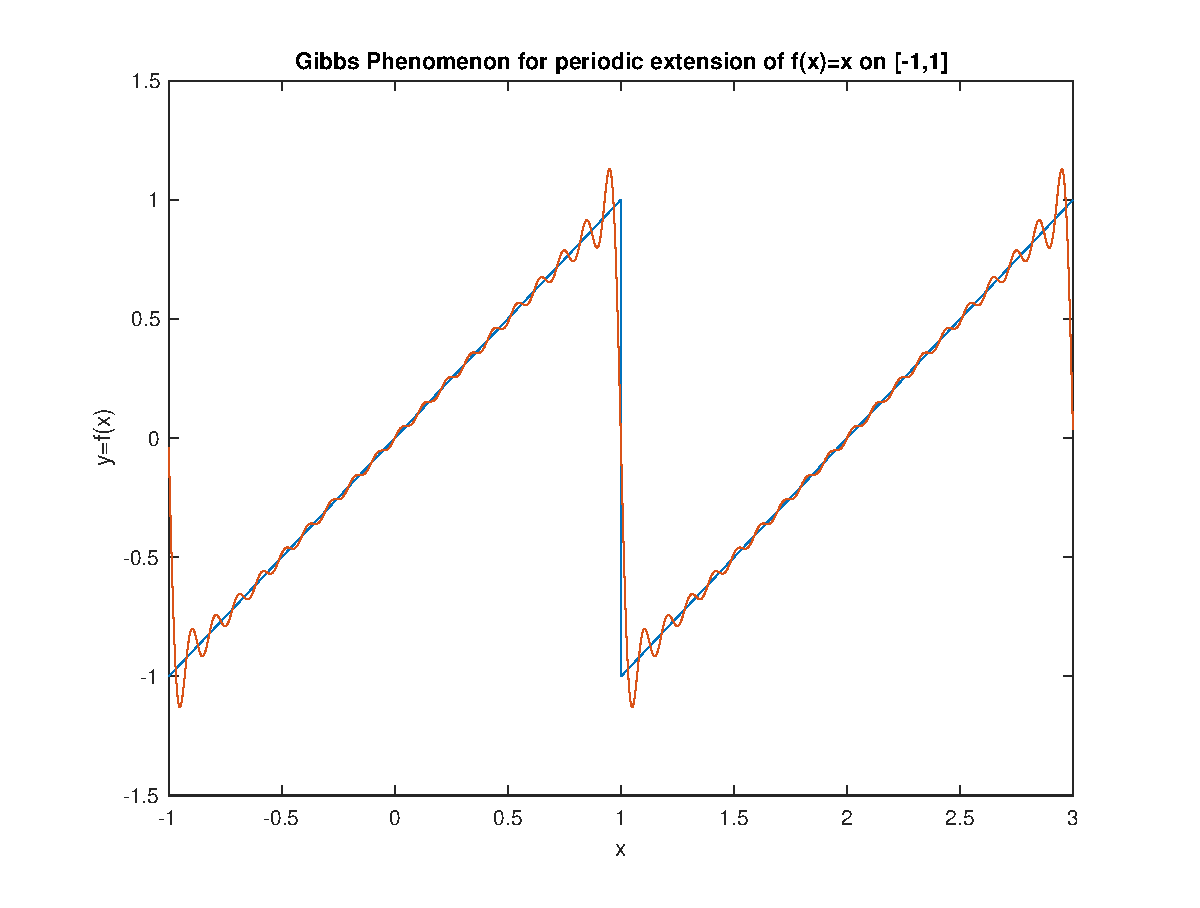
\includegraphics[scale=.25]{Gibbs.eps}
\end{figure}
\item Goal of Fourier Continuation is to get the similar accuracy, convergence, and computational cost with non-periodic functions
\item As a result of using Fourier Continuation approximations, we are given periodic extensions of smooth functions that can be used in conjunction with FFTs to compute numerical solutions to differential equations.
\end{itemize}
}
\frame{
\normalsize
\frametitle{Construction}
\small
Given a smooth function $y=f(x)$ on $[0,1]$ where $f \in C^k[0,1]$, $k>0$.  Discretize the interval onto $N$ points and let $x_j$ be the $j^{\text{th}}$ point on the interval with corresponding function value $y_j=f(x_j)$. 
Choose period $b>1$, and expand in terms of $M$ Fourier Modes, $M<N$, and the problem to solve becomes 
\begin{eqnarray}
y_j=\sum_{k\in t(M)} a_k e^{\dfrac{2\pi i}{b}kx_j}, &j=1\ldots N
\end{eqnarray}
\cite{FC1}. As an example, consider $f(x)=x$ on $[0,1]$.  We discretize on $16$ points, let $b=2$, and $M=7$.  A resulting Fourier Continuation approximation for $f$ is
\begin{figure}[h!]
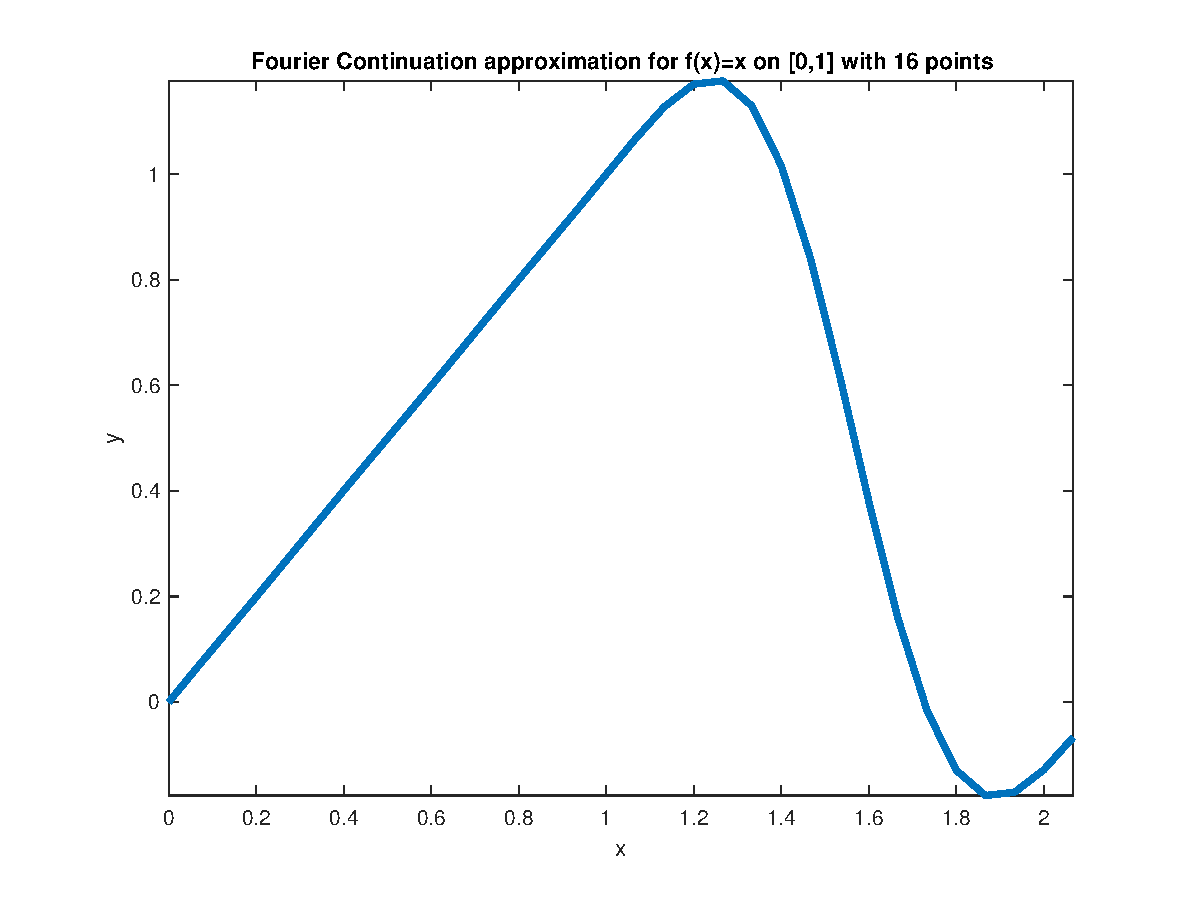
\includegraphics[scale=.25]{FCEx.eps}
\end{figure}

}
\subsection{FC-Gram}
\frame{
\frametitle{FC-Gram}
\begin{itemize}
\item Begin with a basis of polynomials on $n$ points, $f_0,f_1,\ldots,f_{n-1}$
\item Create and store the Fourier Continuation approximations for each of the polynomials
\item Given a function $f$ on any interval with any number of points $m$, sample the first $n$ points and the last $n$ points of $f$.  If $m=n$, use the same $n$ points in order. 
\item Fit the first $n$ points to the basis and the last $n$ points to the basis separately, giving us coefficient vectors $a_1$ and $a_2$ respectively.
\item An appropriate combination of $a_1$ and $a_2$ applied to the continuations of their respective polynomials is taken to get a smooth, periodic extension of $f$
\end{itemize}
}

\frame{
\frametitle{FC-Gram Example}
\begin{figure}[h!]
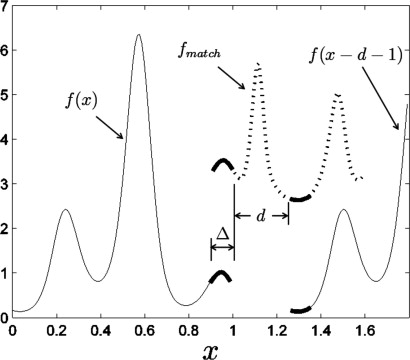
\includegraphics[scale=.5]{FCGram.jpg}
\caption{A comprehensive picture of the FC-Gram method as applied to $f(x)=e^{\sin(5.4\pi x-2.7\pi)-\cos(2\pi x)}$\cite{FCAD1}}
\end{figure}
}
\section{Current Work}
\frame{\frametitle{Multiple Continuation approximations}
As explained in the Fourier Continuation section, there are several possible Fourier Continuation approximations for the same function.  
\begin{figure}[h!]
\begin{center}
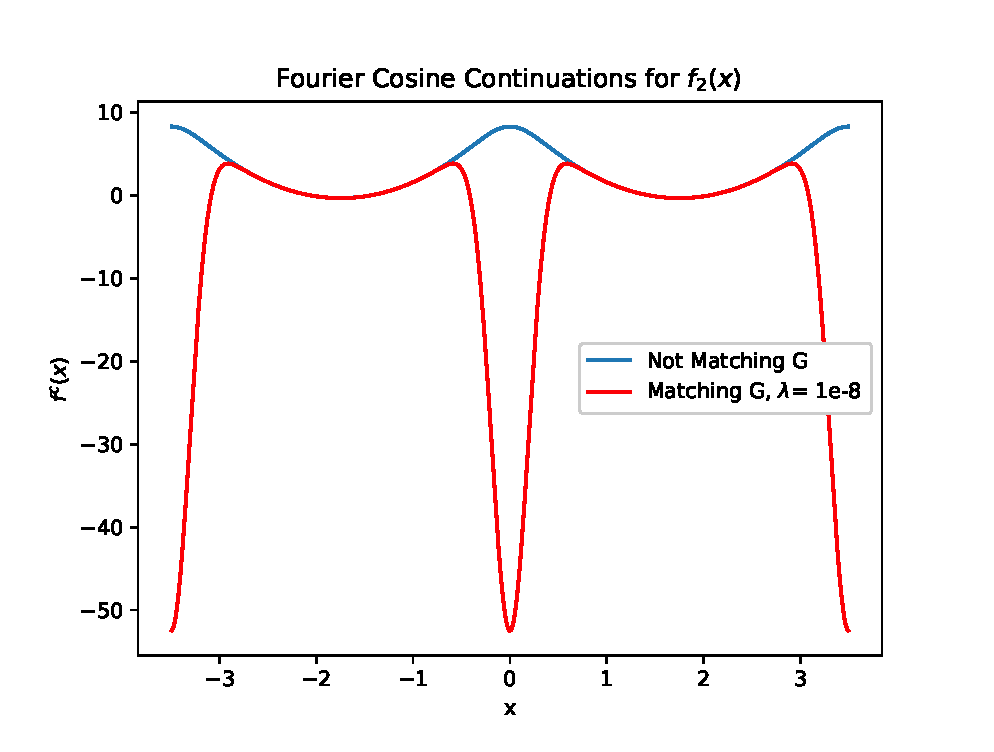
\includegraphics[scale = .3]{f_2ForComparison.eps}
\end{center}
\end{figure}
\normalsize
By adding constraints to the system of equations, we can control the shape of the continuation and ultimately create a stable approximation.  
}
\subsection{Green's Function Solution}
\frame{\frametitle{Green's Function Solutions}
Matching the differential operator to the Green's Function solutions for the given BVP is a natural choice.  The Green's Function solutions are inherently stable under the $\infty$-norm and thus provide the beginning steps for the new form the continuations will take.  
\begin{itemize}
\item Compute the Green's Function for the differential equation $-\alpha u'' + u = f$, $u(x_{\ell})=0$, $u(x_r)=0$. This yields $G(x,a)$ \cite{BO}.
\item Compute the Green's Function solution as $\displaystyle \int_{x_{\ell}}^{x_r} G(x,a)f(a)da$.  
\end{itemize}
}
\frame{
The homogeneous solutions used to calculate the Green's function for the given BVP with $x_{\ell}=-1$, $x_r=b$ are
\begin{eqnarray}
h_1(x) &=& e^{\frac{(x-b)}{\sqrt{\alpha}}} \\
h_2(x) &=& e^{\frac{(-x-1)}{\sqrt{\alpha}}},
\end{eqnarray}

The calculated Green's Function for $x_{\ell}=-1$, $x_r=b$ is
\tiny
\begin{equation}
G(x,a)=\begin{cases} 
-\dfrac{1}{2} \dfrac{\sqrt{\alpha}\left(-e^{\frac{-1-2b+a}{\sqrt{\alpha}}}+e^{-\frac{a+1}{\sqrt{\alpha}}}\right)\left(-e^{\frac{2(2+b+x)}{\sqrt{\alpha}}}+e^{\frac{2(x+1)}{\sqrt{\alpha}}}+e^{\frac{2(1+b)}{\sqrt{\alpha}}}-1\right)e^{\frac{-x+1+2b}{\sqrt{\alpha}}}}{\left(e^{\frac{2(1+b)}{\sqrt{\alpha}}}-1\right)^2} & x<a \\
\dfrac{1}{2} \dfrac{\sqrt{\alpha} \left(e^{\frac{2+b+a}{\sqrt{\alpha}}} -e^{\frac{a-b}{\sqrt{\alpha}}}\right)\left(e^{\frac{2(-x+b)}{\sqrt{\alpha}}}+e^{\frac{2(1+b)}{\sqrt{\alpha}}}-e^{\frac{2+4b-2x}{\sqrt{\alpha}}}-1\right)e^{\frac{2+b+x}{\sqrt{\alpha}}}}{\left(e^{\frac{2(1+p)}{\sqrt{\alpha}}}-1\right)^2} & x \geq a

\end{cases}
\end{equation}
}
\normalsize
\subsection{Minimization Problem}
\frame{
\begin{itemize}
\item Given $n$ points on an interval, we construct the Gram polynomials $f_0,f_1,\ldots,f_{n-1}$.  Then a sine or cosine continuation matrix is created on a grid, and the functions are evaluated on the same grid. 
\item Next, the function $\tilde{f}$ and its cosine (or sine) continuation $C_u$ are matched, which is the equivalent of solving
\begin{equation}
\min ||C_u f^c - \tilde{f} ||^2 .
\end{equation}
\end{itemize}
}
\frame{
This results in an accurate, but generally unstable approximation:
\begin{figure}
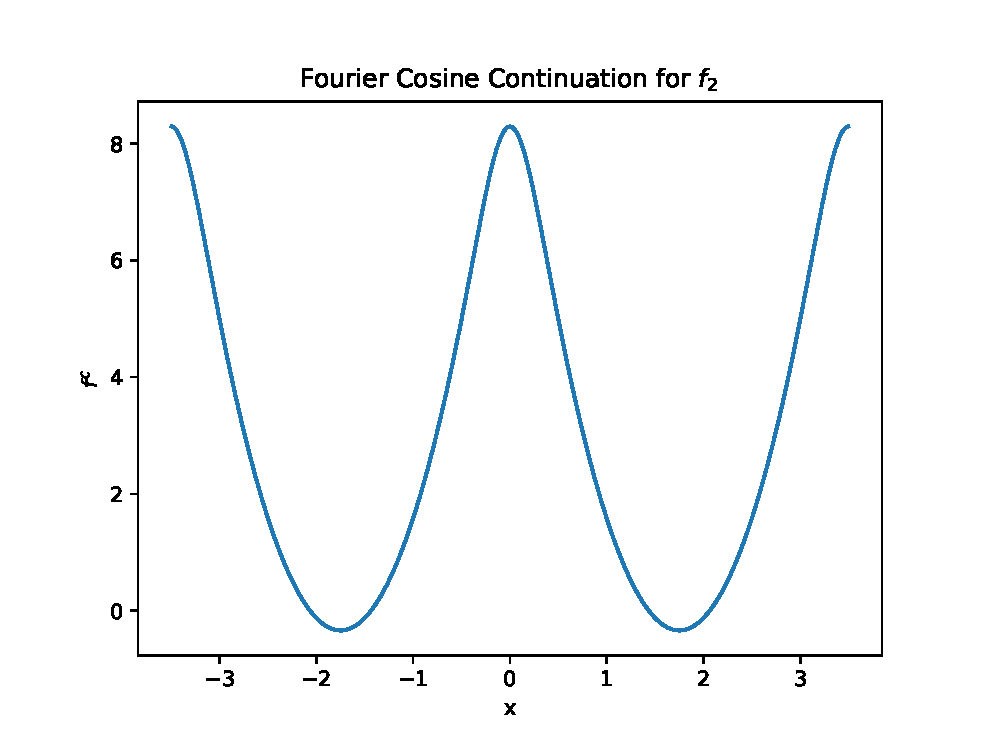
\includegraphics[scale=.4]{f_2NoG.eps}
\end{figure}
}
\frame{
\frametitle{Minimization Problem 2}
\begin{itemize}
\item Using symbolic representations, the Green's function solutions for each of the polynomials are computed and evaluated on the grid. Then a numerical differential operator $I-\alpha\dfrac{\partial^2}{\partial x^2}$ is created for the sine or cosine continuation. 
\item We constrain the original minimization problem using the Green's function and the inverted differential operator applied to the continuation. This yields
\begin{equation}
\min ||C_u f^c - \tilde{f}|| ^2 + ||C_u D_c^{\dagger} f^c - \tilde{G}||^2
\end{equation} 
\end{itemize}
}
\frame{
While this approximation is stable, it loses accuracy. 
\begin{figure}
\begin{tabular}{c}
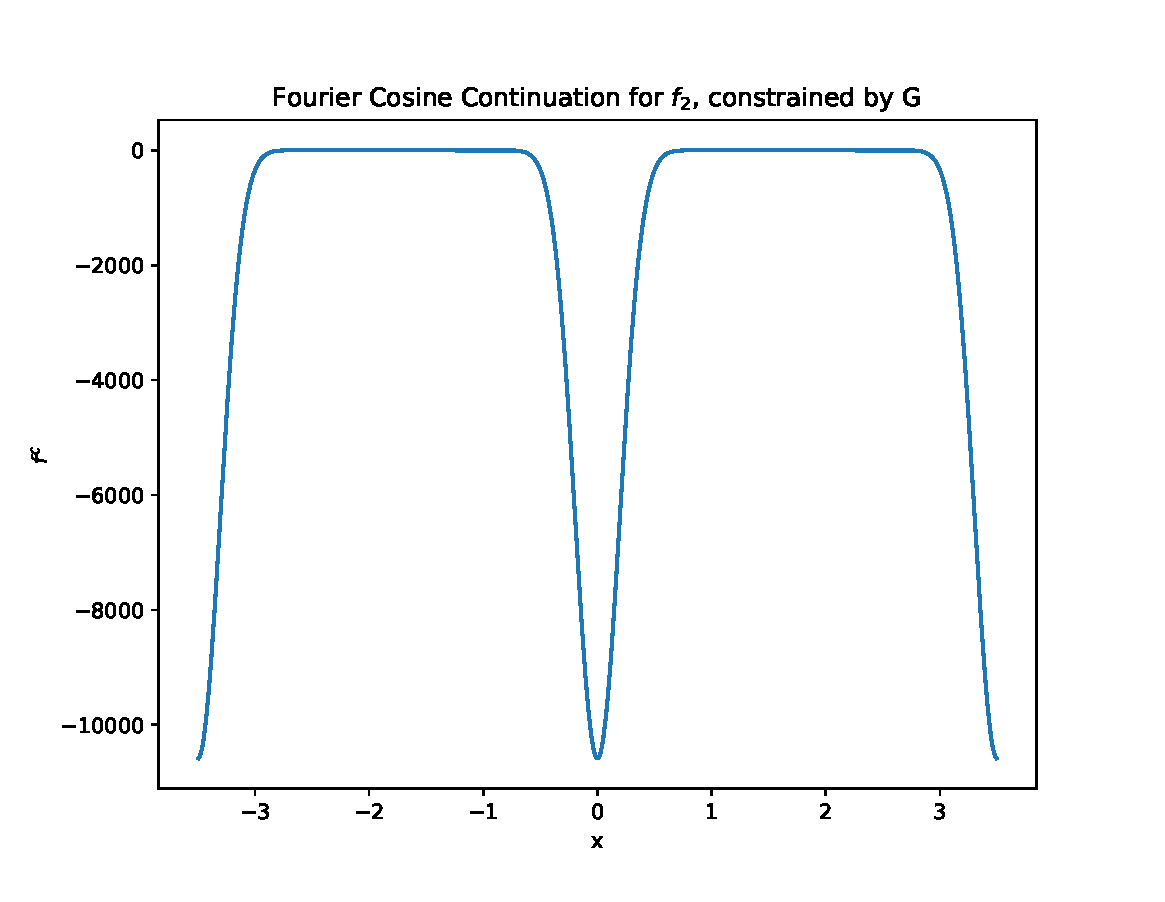
\includegraphics[scale=.3]{f_2WGNoH.eps} \\
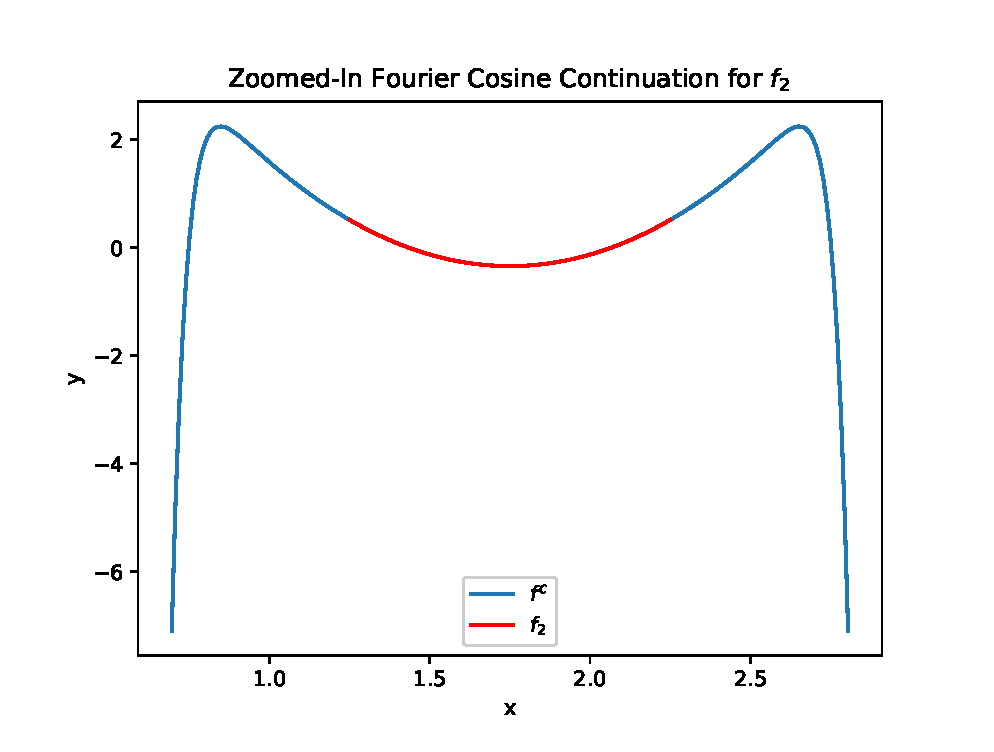
\includegraphics[scale=.3]{f_2NoHZoom.eps}
\end{tabular}
\end{figure}


}

\frame{
\frametitle{Minimization Problem 3}
In practice, solving this minimization problem does not achieve great accuracy nor stability.  The homogeneous solutions are not well-represented in the Fourier basis, but the Green's function solution is created from them. An additional constraint is needed in order to allow the system to accurately represent the function while separating out the homogeneous solutions.  Including this constraint modifies the system to
\begin{equation}
\min ||C_u f^c - \tilde{f}|| ^2 + ||C_u D_c^{\dagger} f^c +c_1 \tilde{h_1} + c_2 \tilde{h_2} - \tilde{G}||^2
\end{equation}
where $c_1$ and $c_2$ will be chosen by the computational method to achieve greatest accuracy in the least-squares sense. 
}
\frame{
This gives accuracy, but trades off on stability.  
\begin{figure}
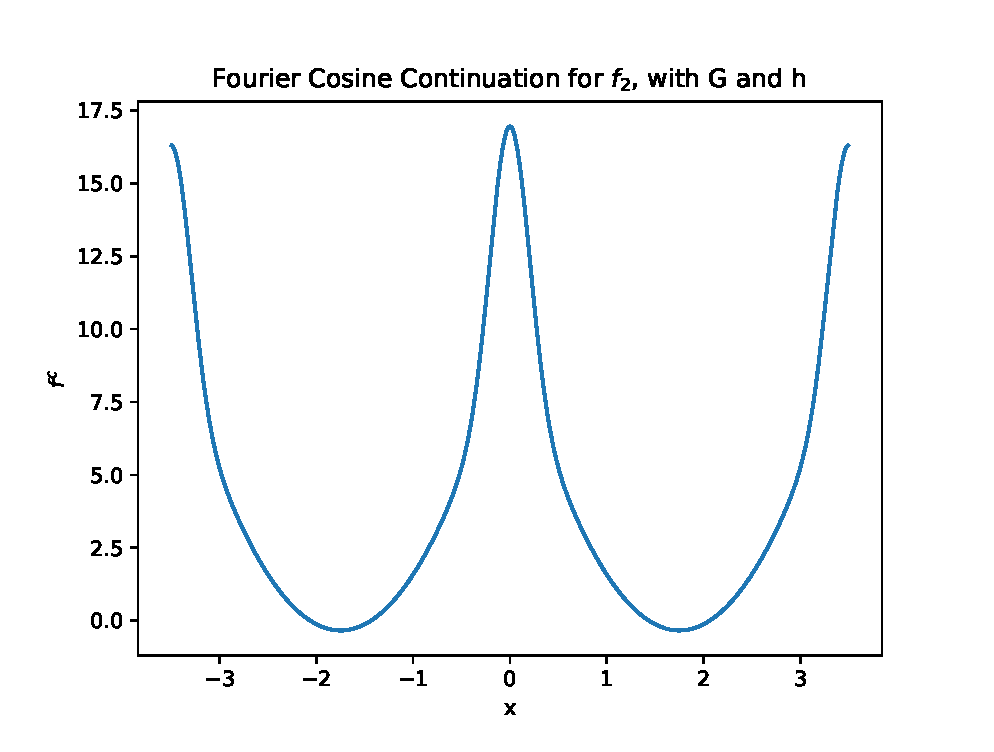
\includegraphics[scale=.4]{f_2WGWGNoL.eps}
\end{figure}

}

\frame{
\frametitle{Minimization Problem 4}
Lastly, two other parameters $\lambda$ and $\mu$ which force the continuations $f^c$ to be stable.  The first, $\lambda$, is applied to control the magnitude of $c_1$ and $c_2$ relative to the homogeneous solutions.  The second, $\mu$ is applied to the coarse-grid point values of the differential operator to control the magnitude of the continuation under the derivative. The final minimization problem we have is
\begin{equation}
\begin{aligned}
\min ||C_u f^c - \tilde{f}|| ^2 + ||C_u D_c^{\dagger} f^c +c_1\tilde{h_1}+c_2\tilde{h_2}- \tilde{G}||^2 \\+ \lambda^2|| c_1 \tilde{h_1} + c_2 \tilde{h_2} ||^2 + \mu^2||C_u D_c^{\dagger}|{\text{\tiny{coarse}}}  ||^2
\end{aligned}
\end{equation}
}
\frame{
\begin{figure}
\includegraphics[scale=.4]{f_2Final.eps}
\end{figure}
}
\subsection{Results}
\frame{
\frametitle{Implementation}
We implement this solver in Julia, using 200 bits of precision in \texttt{BigFloat}.  For 200 bits, $\epsilon \approx 10^{-77}$.  With the conditioning of the system, having 77 digits of precision mitigates great error propagation.  The Julia packages \texttt{GenericSVD}, \texttt{SymPy}, and \texttt{PyPlot} were used.  To find the least-squares solution to our minimization problem, we used an SVD and found the pseudoinverse with a tolerance of $10^{-40}$.
}
\frame{
\frametitle{Implementation 2}
Let $n$ be the number of points on a coarse grid unit interval, coinciding with the number of points the Gram polynomials are computed on.  Let $F$ be the factor by which the coarse grid is refined, so if the original spacing is $h=\frac{1}{n-1}$, the fine grid spacing will be $h_f=\frac{1}{(n-1)\times F}$.  While calculations are performed on a full double period ($2b$), measurable results are only calculated on the unit interval.\\
\vspace{.2in}
Accuracy was measured as
\begin{equation}
a=\| f^c|_{\text{\tiny{fine}}}-f|_{\text{\tiny{fine}}}\|_2
\end{equation}
and stability was measured as
\begin{equation}
s=\frac{\|u^c|_{\text{\tiny{coarse}}}\|_2}{\|f|_{\text{\tiny{coarse}}}\|_2}
\end{equation}
}
\frame{
\frametitle{Some Results}
Letting $n=10$, $b=3.5$ and setting the unit interval from $1.25$ to $2.25$ the evaluation of the Gram polynomials and the corresponding Green's function solutions were shifted accordingly .  The coarse grid of 10 points was refined by a factor of 10 to give a fine grid of 100 points.  Stability was achieved with great accuracy for various values of $\alpha$.  
}
\frame{
\frametitle{Some Results}
Here are two cosine continuations for $f_0$ and $f_1$ with $\alpha = 0.001$:
\begin{figure}[h!]
\centering
\begin{tabular}{|c|c|}
\hline
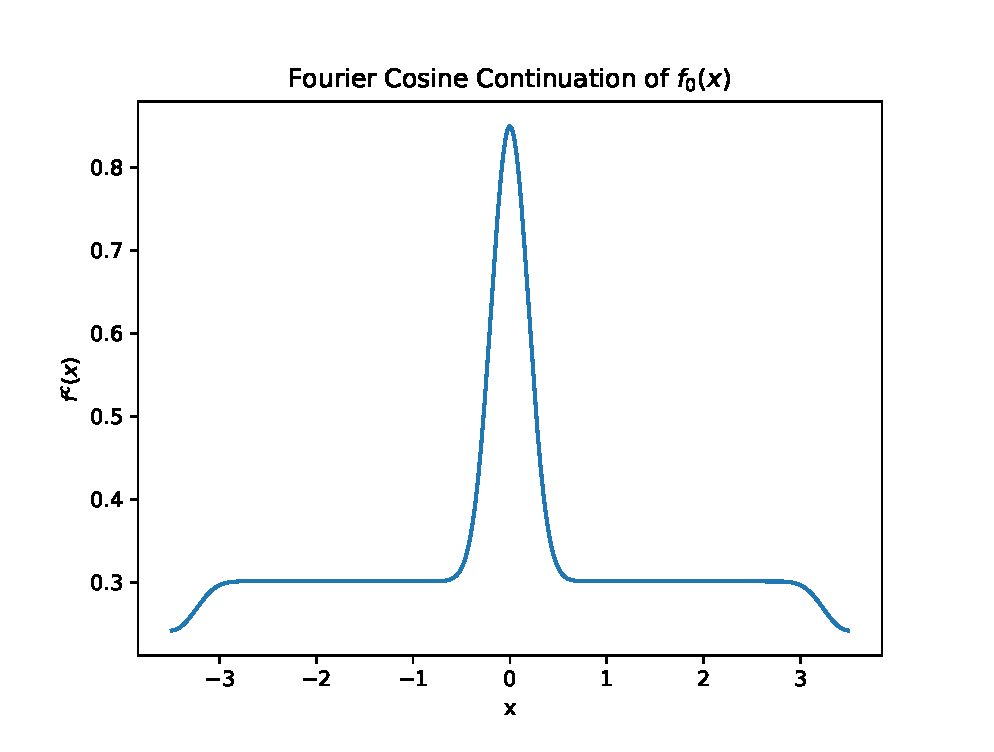
\includegraphics[scale=.25]{f_0Cosine.eps}

&
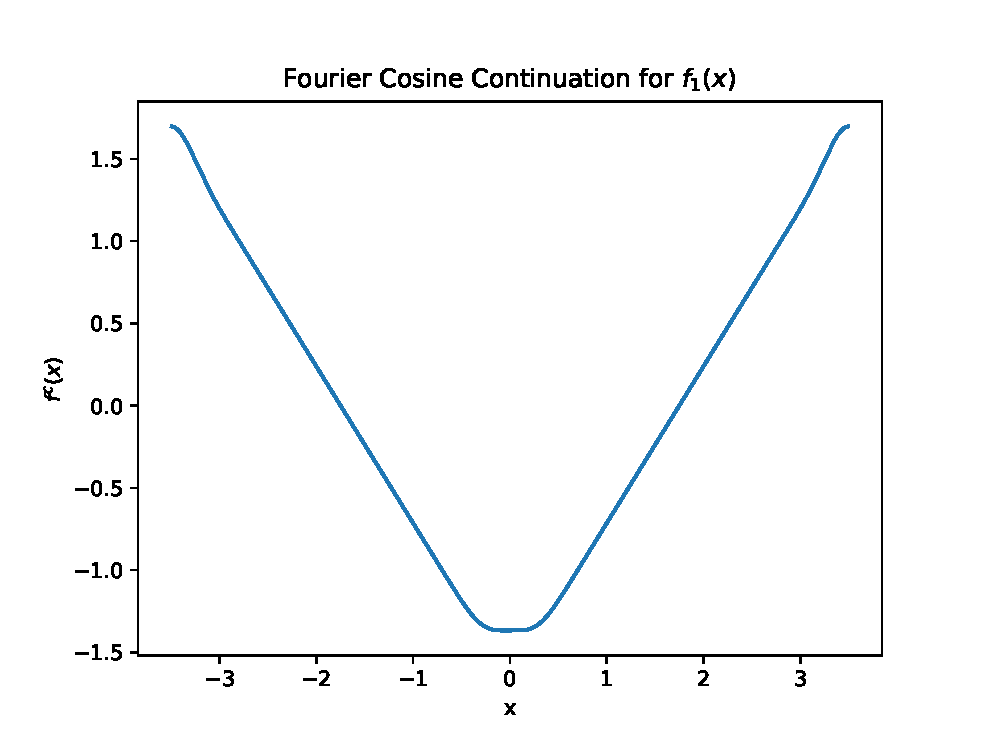
\includegraphics[scale=.25]{f_1Cosine.eps}\\
\hline


\end{tabular}
\end{figure}
}
\frame{
\frametitle{Some Results}
Here is a cosine continuation for $f_1$, accompanied by the computed solution $u$, for $\alpha = 0.01$
\begin{figure}[h!]
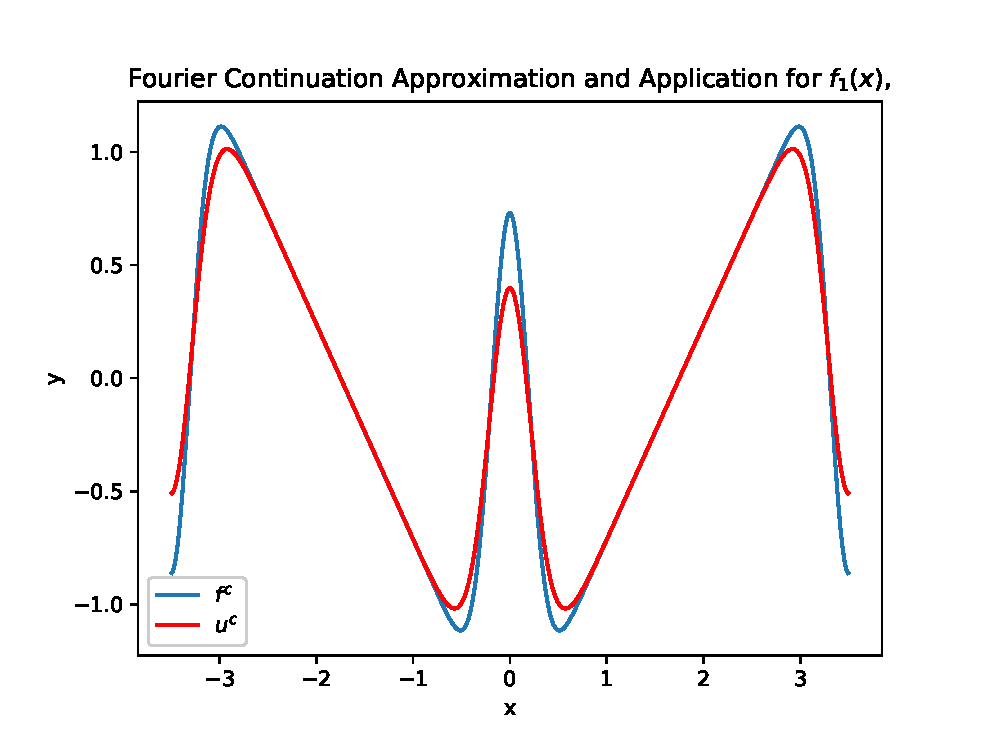
\includegraphics[scale=.45]{f_1u_1.eps}
\end{figure}
}
\frame{
\frametitle{Some Results}
Here is a sine continuation for $f_2$, accompanied by the error for the unit interval a for $\alpha=0.01$ with $\lambda = 3.59\times 10^{-14}$.  This is a stable approximation. 
\begin{figure}
\begin{tabular}{c c}

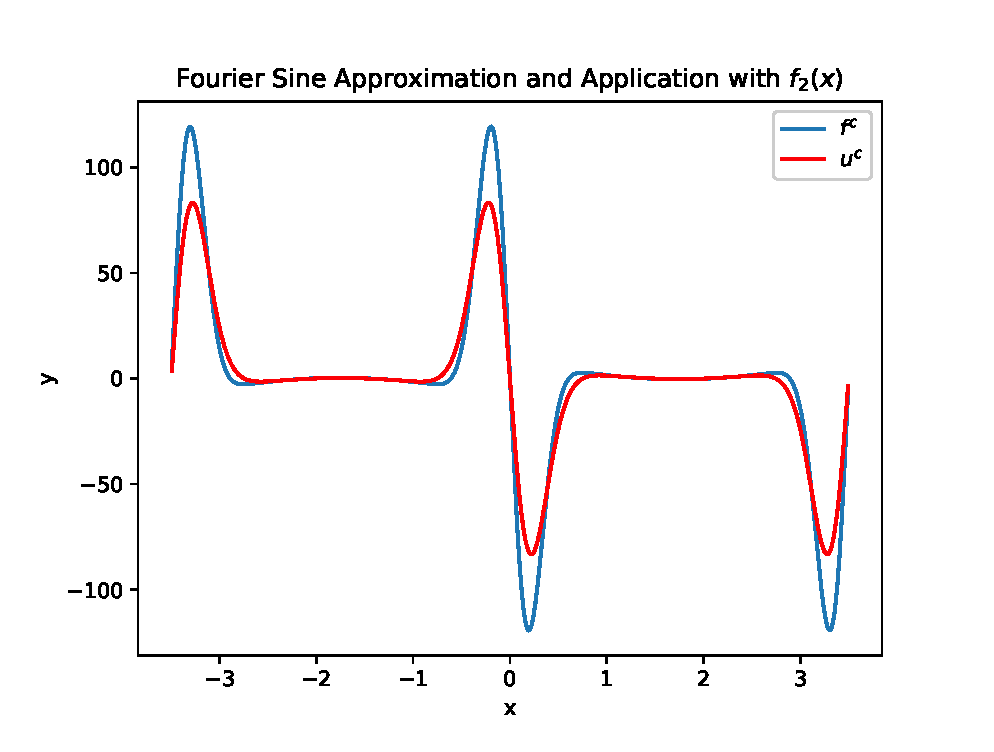
\includegraphics[scale=0.3]{f_2Sinewu.eps}

& 
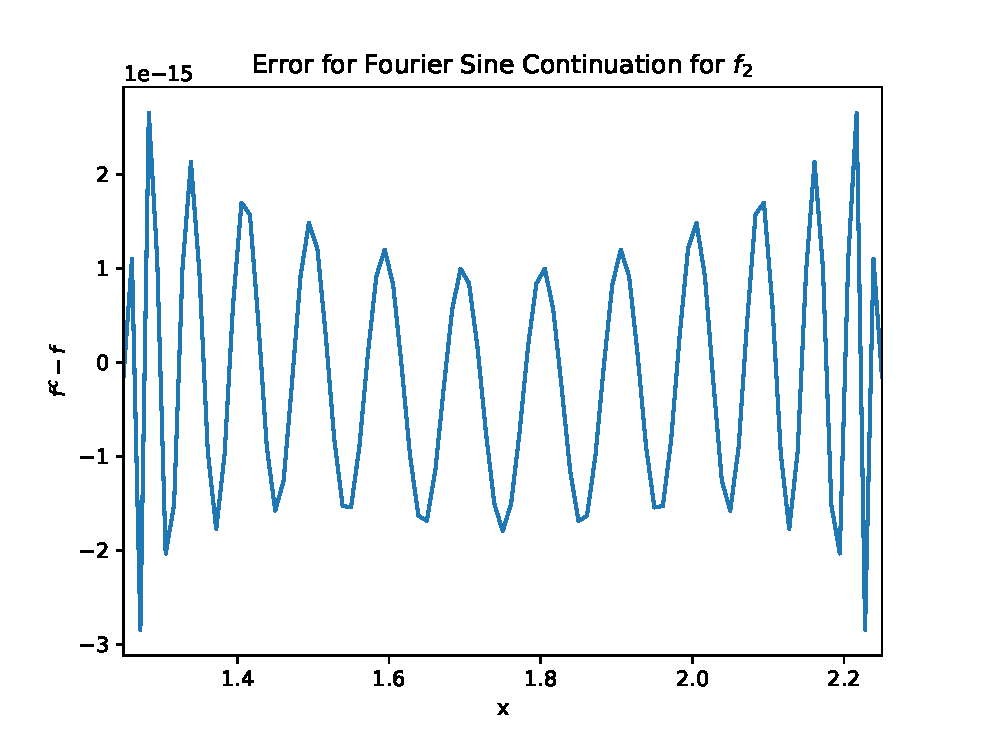
\includegraphics[scale=0.3]{Errorf_2Sine.eps}
\end{tabular}
\end{figure}
}
\frame{
\frametitle{Some Results}
To better view how the sine continuation matches the function, here is a zoomed in view of $f_2$, $f^c_2$ and the accompanying solution $u$ for $\alpha=0.01$ with $\lambda = 3.59\times 10^{-14}$, on the unit interval $f_2$ is originally defined on:
\begin{figure}
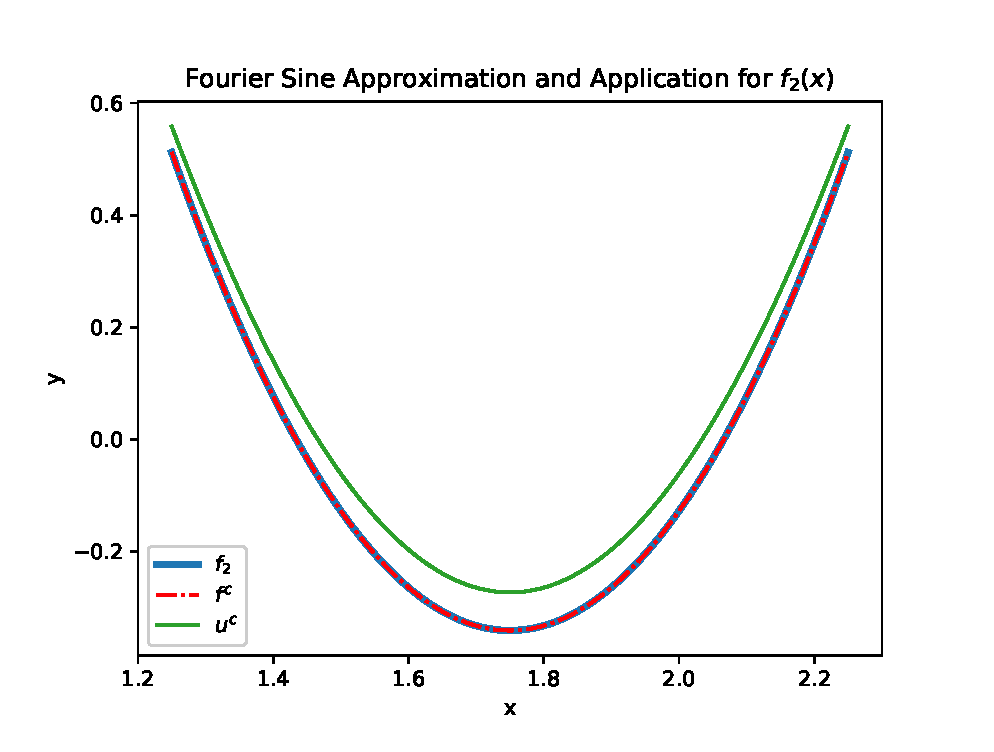
\includegraphics[scale=0.4]{f_2u_2unit.eps}
\end{figure}
}
\frame{
\frametitle{Predicting $\lambda$ and $\mu$ given $\alpha$}
The stability of the approximations is dependent on $\alpha$.  To be able to use this method as a fast method, the form of the continuation must be easily predicted for any given $\alpha$.  The first approach taken was to find a value of $\lambda$ that gives stability up to a tolerance.  This was achieve with a bisection method for values of $\lambda$ between $10^{-20}$ and $10^0$. \\
For Fourier Cosine continuations with $\alpha=0.001$, the optimized $\lambda$ values are listed with the corresponding measure of accuracy and stability for each polynomial:
\tiny
\begin{tabular}{|c|c|c|c|}
\hline & & &\\
Degree & $\lambda$ & Accuracy& Stability \\ \hline  & & & \\
0 & $3.255881466810751\times 10^{-13}$ & $2.86510896623681\times 10^{-17}$ & $0.999999999999$ \\ \hline  
1 & $1.839023251669854\times 10^{-13}$ & $3.92206770433105\times 10^{-17}$ & $0.999999999999$ \\ \hline  
2 & $1.4852300108136326\times 10^{-10}$ &  $3.88957362362112\times 10^{-12}$ & $0.999999999999$ \\ \hline 
3 & $5.518469567738165\times 10^{-10}$ & $5.61719253880104\times 10^{-11}$ & $0.999999999999$ \\ \hline 
4 & $1.1767778737499883\times 10^{-9}$ & $2.0963541751156\times 10^{-10}$ & $0.999999999999$ \\ \hline 
5 & $3.0091447070493457\times 10^{-9}$ & $1.4098065193636\times 10^{-9}$ & $0.999999999999$ \\ \hline 
6 & $4.864688165149565\times 10^{-9}$ & $3.1835304451683\times 10^{-9}$ & $0.999999999999$ \\ \hline 
7 & $1.0373945031909215\times 10^{-8}$ & $1.52729276442667\times 10^{-8}$ &  $0.999999999999$ \\ \hline
8 & $1.5639865553913073\times 10^{-8}$ & $3.08554433657289\times 10^{-8}$ & $0.999999999999$  \\ \hline
9 & $3.071964692890429\times 10^{-8}$ & $1.72857119028618\times 10^{-7}$& $0.999999998446$  \\ \hline
\end{tabular}  
}
\frame{
\frametitle{Controlling the Continuation Size}
As a result of maximizing stability, the magnitude of the continuations becomes large.
\begin{figure}
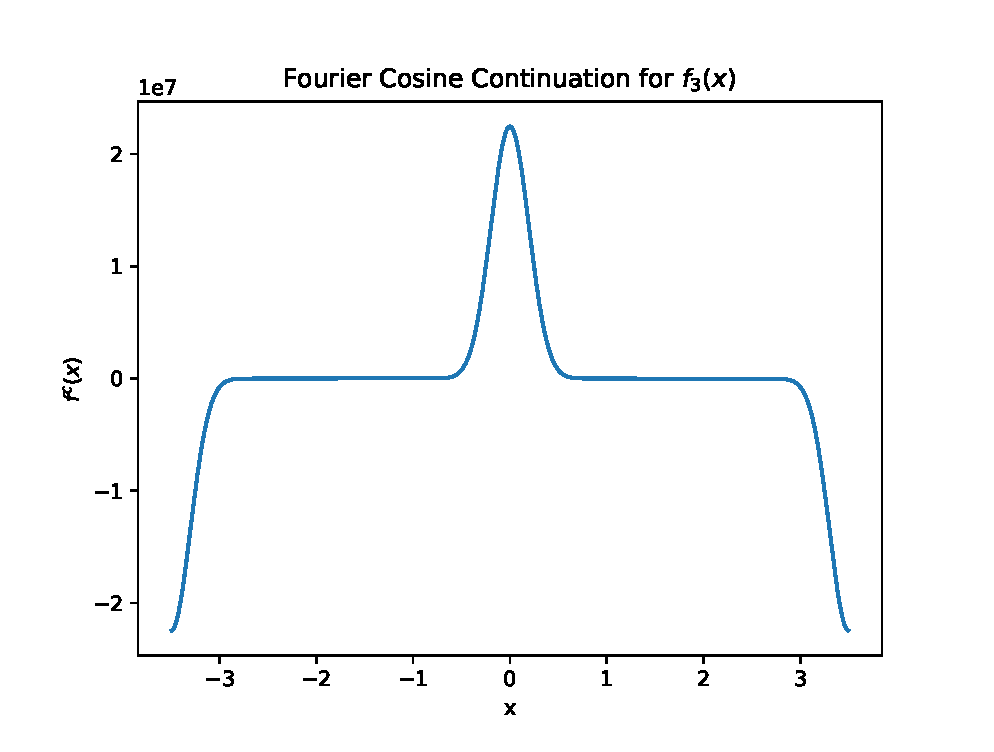
\includegraphics[scale=.3]{f_3Cosine.eps}
\end{figure}
This is not ideal for implementation in other programming languages as the magnitude will affect the number of digits of accuracy that can be maintained when using a language that has $\epsilon<10^{-77}$.  
}

\section{Future Work}
\frame{
\begin{itemize}
\item Now that stability is an achievable result, we hope to find a predictor such that a continuation can be stored and chosen based on the value of $\alpha$ used, without solving a system every time
\item After the basis is stored, the FC-Gram method will be applied to several test functions, including the Runge function, in order to determine the accuracy of the method in implementation with any input of data
\begin{itemize}
\item At this point, the FC-Gram method will be applied first on $n$ points, and then increasing the number of points to get an error estimate as the number of points gets large. 
\end{itemize}
\item Next, BVPs with various BCs with be solved using the continuations and FC-Gram. 
\item Lastly, this will be implemented in PDEs as the BVP-solver in the time stepping of the FC-AD method
\end{itemize}
}
\frame{
\begin{itemize}
\item A convergence estimate is needed first and foremost.  It has been shown in \cite{Platte} that convergence of fast stable approximations on equispaced points is impossible, therefore the convergence estimates speaks to maximal errors as step size decreases instead of taking a limit.  
\item Formal justification of the stability of this method is needed. 
\end{itemize}
}


\section{References}
\frame{
\frametitle{References}
\scriptsize
\bibliographystyle{unsrt}
\bibliography{citations}
}



\end{document}
